% !TeX root = ../tesis.tex
%%%%%%%%%%%%%%%%%%%%%%%%%%%%%%%%%%%%%%%%%%%%%%%%%%%%%%%%%%%%%%%%%%%
% SECCIÓN: FUNDAMENTOS DE LA TEORÍA DE GRAFOS E IMPLEMENTACIÓN
%%%%%%%%%%%%%%%%%%%%%%%%%%%%%%%%%%%%%%%%%%%%%%%%%%%%%%%%%%%%%%%%%%%
\section{Grafos Matemáticos y su Implementación Computacional}
\label{sec:grafos-matematicos}

\subsection{Origen y Fundamentos: La Abstracción de Euler}
\label{subsec:euler}
    El estudio formal de la teoría de grafos se remonta a 1736, cuando Leonhard Euler publicó su resolución al
    problema de los siete puentes de la ciudad de Königsberg. El núcleo de ese aporte residió en la capacidad de
    abstraer la geografía física de la ciudad ---dividida por el río Pregel en cuatro zonas terrestres--- hacia un
    esquema puramente relacional: las zonas se representaron como puntos (vértices) y los puentes como líneas
    (aristas), de modo que el problema se resolviera no mediante la geometría física, sino a través de la
    configuración topológica del sistema, tal como se aprecia en la Figura~\ref{fig:königsberg}
    \parencite{garcia2005, braicovich2009}.

\begin{figure}[H]
    \centering
    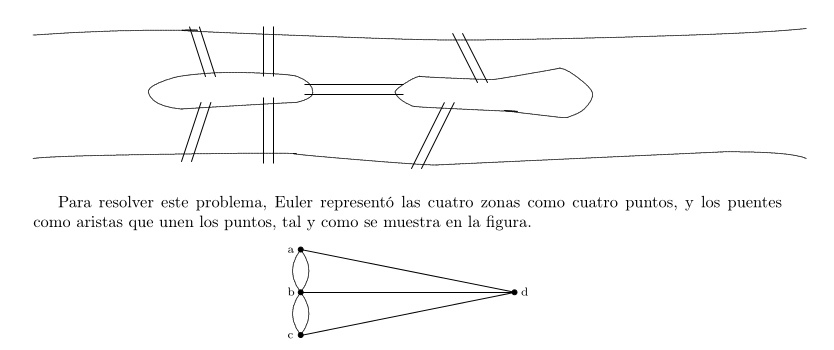
\includegraphics[width=0.70\textwidth]{Figures/Cap3/MapaKonisnberg.png}
    \caption{Mapa histórico de Königsberg y su representación como grafo}
    \label{fig:königsberg}
    \fuentefigura{Figura extraída de \textcite{garcia2005}.}
\end{figure}

\subsection{Grafos de Euler y la Condición de Transitabilidad}
\label{subsec:grafos-euler}
    Derivado del trabajo fundacional de Euler, se establece que un grafo es euleriano si admite un circuito que
    recorra todas sus aristas exactamente una vez, regresando al vértice de origen. La condición necesaria y
    suficiente para que un grafo conexo admita este recorrido es que todos sus vértices posean un grado par; si el
    grafo posee exactamente dos vértices de grado impar, admite en cambio un camino de Euler abierto, que debe
    comenzar en uno de esos vértices y terminar en el otro. Ambas configuraciones se ilustran comparativamente en
    la Figura~\ref{fig:diagramas-aristas} \parencite{garcia2005, braicovich2009}. Esta distinción resulta
    fundamental en problemas de transporte y logística como el del ``cartero chino'', donde se busca minimizar el
    costo de un recorrido que cubra toda una infraestructura vial \parencite{allauca2023}.

\begin{figure}[H]
    \centering
    \begin{subfigure}[b]{0.47\textwidth}
        \centering
        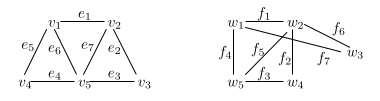
\includegraphics[width=\textwidth]{Figures/Cap3/Diagrama1Aristas.png}
        \caption{Representación esquemática de un grafo}
        \label{fig:DiagramaAristas1}
    \end{subfigure}
    \hfill
    \begin{subfigure}[b]{0.47\textwidth}
        \centering
        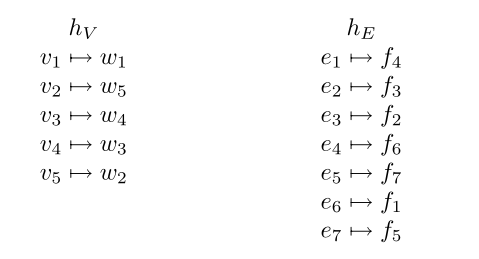
\includegraphics[width=\textwidth]{Figures/Cap3/Diagrama2Aristas.png}
        \caption{Nodos, aristas y condiciones de grado}
        \label{fig:DiagramaAristas2}
    \end{subfigure}
    \caption{Elementos constitutivos de un grafo y condiciones de transitabilidad euleriana}
    \label{fig:diagramas-aristas}
    \fuentefigura{Figuras extraídas de \textcite{garcia2005}.}
\end{figure}

\subsection{Grafos Computacionales: Eficiencia mediante Mapas de Adyacencia}
\label{subsec:grafos-computacionales}
    En el ámbito de las ciencias de la computación, existe una distinción operativa entre el grafo como ente
    matemático abstracto y su implementación en sistemas de datos. \textcite{valiente2022} sostiene que, si bien
    las representaciones tradicionales como las matrices de adyacencia ofrecen un acceso rápido, suelen ser
    ineficientes en el uso de memoria para grafos dispersos. Como alternativa superior, se destacan los
    \textbf{Mapas de Adyacencia (\termino{Adjacency Maps})}, estructuras que particionan nodos y aristas mediante
    diccionarios indexados y permiten verificar la adyacencia entre dos nodos en un tiempo esperado constante
    $O(1)$, optimizando así el rendimiento de los algoritmos en redes de gran escala, tal como se esquematiza en
    la Figura~\ref{fig:PresentacionCaminos}.

\begin{figure}[H]
    \centering
    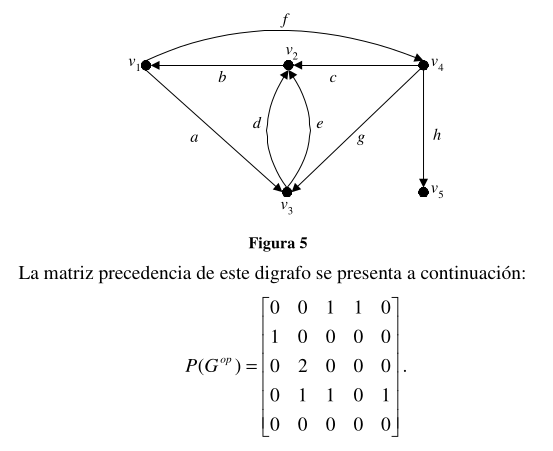
\includegraphics[width=0.75\textwidth]{Figures/Cap3/RepresentacionCaminos.png}
    \caption{Representación matemática de caminos sobre una matriz de adyacencia}
    \label{fig:PresentacionCaminos}
    \fuentefigura{Figura extraída de \textcite{braicovich2009}.}
\end{figure}

\subsection{Optimización de Redes: El Cálculo de Caminos Mínimos}
\label{subsec:caminos-minimos}
    La aplicación de la teoría de grafos en la optimización logística permite resolver desafíos complejos de
    enrutamiento. \textcite{allauca2023} expone que las redes de transporte pueden modelarse como grafos dirigidos
    valorados, donde los nodos representan estaciones y las aristas son rutas ponderadas por variables como tiempo
    y costo. Bajo este enfoque, se destacan algoritmos fundamentales como el de \dijkstra{} para hallar el camino
    más corto desde un nodo origen, y el de \floyd{} para calcular distancias mínimas entre todos los pares de
    nodos, tal como se ilustra en la Figura~\ref{fig:CaminosMinimo}. Estudios de caso demuestran que la aplicación
    de estas técnicas permite reducciones estimadas del 8\% en tiempos de entrega y del 5\% en costos operativos
    \parencite{allauca2023}.

\begin{figure}[H]
    \centering
    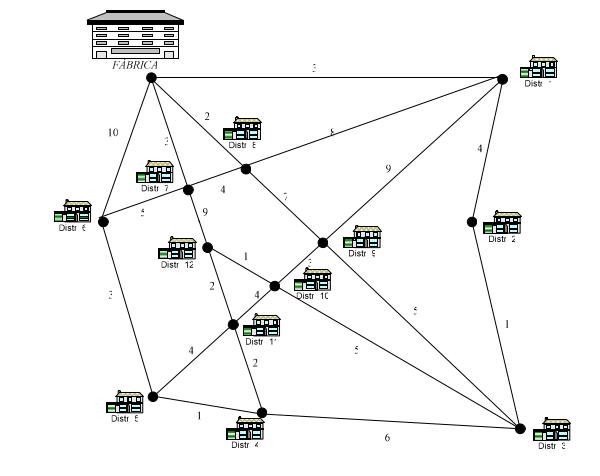
\includegraphics[width=0.75\textwidth]{Figures/Cap3/CaminosMinimos.png}
    \caption{Representación esquemática de caminos mínimos en un problema teórico}
    \label{fig:CaminosMinimo}
    \fuentefigura{Figura extraída de \textcite{braicovich2009}.}
\end{figure}

\subsection{Integración de Grafos con Sistemas \gis{} y Datos \gtfs{}}
\label{subsec:grafos-sig-gtfs}
    La convergencia entre la teoría de grafos y los Sistemas de Información Geográfica (\gis{}) permite un
    análisis avanzado de la conectividad urbana. \textcite{fortin2016innovative} y \textcite{adas2013} proponen
    el uso del estándar \textbf{Google Transit Data (\gtfs{})} como fuente primaria para construir grafos
    dinámicos que integran la topología de la red con su ubicación georreferenciada. Esta convergencia permite
    generar indicadores clave de desempeño, como el \textbf{Detour Factor ($DI$)}, que cuantifica la eficiencia
    geométrica del trazado comparando la distancia real en la red contra la distancia euclidiana; asimismo, el
    uso de modelos de grafos expandidos en el tiempo facilita la evaluación de la accesibilidad dinámica
    considerando frecuencias reales y penalizaciones por transferencia \parencite{fortin2016innovative, adas2013}.

\subsection{Implementaciones Tecnológicas y Algoritmos de Búsqueda}
\label{subsec:implementaciones-grafos}
    En el entorno industrial moderno, las teorías de búsqueda en grafos se implementan a través de motores
    analíticos especializados que procesan datos masivos. \textcite{wang2025} destaca que algoritmos como la
    Búsqueda en Anchura (\termino{BFS}), la Búsqueda en Profundidad (\termino{DFS}) y el algoritmo \termino{A*}
    constituyen el núcleo de las soluciones de navegación actuales. Un ejemplo de esta tendencia es la plataforma
    \textbf{PuppyGraph}, que ofrece una arquitectura de consultas analíticas directamente sobre almacenes de datos
    relacionales, sin procesos de extracción intermedios, y utiliza algoritmos distribuidos para gestionar grafos
    de millones de nodos en aplicaciones de seguridad y logística.
